\graphicspath{{Chapters/Detector/Figures/}}
\chapter{The ATLAS Detector at the LHC}
\label{chap:Detector}

\section{The Large Hadron Collider}

The Large Hadron Collider (LHC) is a particle accelerator located at CERN, the
European Organisation for Nuclear Research, on the French-Swiss border near
Geneva. The LHC is the world's most powerful particle accelerator, colliding beams of
protons together at centre of mass energies of up to 8 \TeV, with the aim of
better understanding the workings of our Universe. It is installed in
tunnel of circumference 26.7 km, which previously held the Large
Electron-Positron Collider (LEP), and is between 45 and 170 m below the ground.
The beams are brought to collisions at four point around the ring, at each of
which a different experiment is located. The machine is also capable of colliding heavy ions, providing a complimentary heavy-ion physics program.

The design of the LHC is described in detail in ~\cite{1748-0221-3-08-S08001}
and ~\cite{Brüning:782076}. A brief summary is given in~\ref{sec-lhc-design},
and details of LHC operations in 2011 and 2012 are given
in~\ref{sec-lhc-operation}.

\subsection{Machine Design}
\label{sec-lhc-design}

The LHC consists of two counter-circulating beams of protons. 
Since the beams are of similarly charged particles
orbiting in opposite directions, they require opposite bending fields, thus need
to be in separate beampipes. Due to space constraints, the two beampipes are
contained within a single structure incorporating a twin bore superconducting
magnet. The magnets must be cooled to 2K to retain their superconducting
properties; this is achieved with a helium based cooling system. Dipole magnets are
used to bend the beams and keep them in orbit. Quadrapole magnets are used to
keep the beams focussed. 

Protons are injected into the LHC from the SPS (Super Proton Synchrotron) in
bunches, at a centre of mass energy of 450 \GeV. They are then accelerated to the desired
collision energy by means of superconducting Radio Frequency (RF) cavities. Once the
particles are accelerated to full energy, the RF cavities are used to keep the
particles in their bunches. The bunches are brought to collision at four points
around the ring, at each of which a different experiment is located. ATLAS sits at
point 1, the ALICE experiment at Point 2, the CMS experiment at Point 5, and the
LHCb experiment at Point 8 (the remaining `Points' are access locations to the
ring).

The rate at which collisions occur depends on the instantanious luminosity
$\mathcal{L}$ and the collision cross-section $\sigma$, related by:

\begin{equation}
\frac{dN}{dt} = \mathcal{L} \cdot \sigma
\end{equation}

The total cross-section for
proton-proton collisions at the LHC has been measured to be
\measStatSyst{98.3}{\errSym{0.2}}{\errSym{2.8}}~mb\footnote{$1 \rm{b} = 10^{-28}
m^{2}$} at a centre of mass energy of 7 \tev~\cite{0295-5075-96-2-21002}. The rate at which a particular
physics process occurs depends on the cross section for the process in question.
Since many of the physics processes under study at the LHC are very rare and
have small cross-sections, it is important to maximise the luminosity as much as
possible.  The instantaneous luminosity can be maximised by increasing the
number of particles per bunch, decreasing the bunch spacing (or equivalently
increasing the number of bunches per beam) or decreasing the size of the bunch
at the interaction point.

% The instantaneous luminosity is given by:

%\begin{equation}
%\mathcal{L} = \frac{N_{\rm{b}}^{2}n_{\rm{b}}f_{\rm{rev}}\gamma_{\rm{r}}}{4\pi
%\epsilon_{n}\Beta^{*}F
%\end{equation}
%
%where $N_{\rm{b}}$ is the number of particles per bunch, $n_{\rm{b}}$ is the
%number of bunches per beam, $f_{\rm{rev}}$ is the revolution frequency

A measure of how many collisions have occured is the integrated luminosity:

\begin{equation}
L = \int \mathcal{L} dt
\end{equation}

The number of events occuring for a given process with cross-section
$\sigma_{\rm{process}}$ is given by:

\begin{equation}
N_{\rm{process}} = L \cdot \sigma_{\rm{process}}
\end{equation}

\subsection{LHC Operation in 2011 and 2012}
\label{sec-lhc-operation}

The LHC began operation in November 2099 with collisions at a centre of mass
energy of 900 \GeV, withe the centre of mass energy raising to a world record
2.36 \TeV\ by the end of the year. In 2010 the centre of mass energy was
succesfully increased to 7 \TeV.
% Say something about the luminosity here
% Say something about int lumi delivered to ATLAS

Details of the LHC operational parameters in 2011 and 2012, together with the
nominal design values, are given in~\tab{lhc-params}.

% Table comparing nominal parameters, 2011, 2012
% E.g. Inst. Lumi, Bunch spacing, # bunches / beam, # protons / bunch

\begin{table}[h!]
\centering
\small
\setlength{\extrarowheight}{4pt}
\begin{tabular}{ l | c | c | c  }
\hline\hline
Parameter & Design & 2011 Operation & 2012 Operation \\
\hline
Proton Energy & 7 \tev\ & 3.5 \tev\ & 4 \tev \\
No. particles per bunch (max) & 1.15 $\times 10^{11}$ & 1.5 $\times 10^{11}$ & 1.6 $\times 10^{11}$  \\
No. of bunches per beam (max) & 2808 & 1380 & 1380 \\
Bunch spacing & 25 ns & 50 ns & 50 ns \\
Peak Luminosity (max) & 1.0 $\times 10^{34} \rm{cm}^{-2}\rm{s}^{-1}$ & 3.6 $\times
10^{33} \rm{cm}^{-2}\rm{s}^{-1}$  & 7.7 $\times 10^{33} \rm{cm}^{-2}\rm{s}^{-1}$ \\
\hline\hline
\end{tabular}
 \caption{LHC operational parameters. A comparison is made of the nominal design
 parameters~\cite{Brüning:782076}, and those used in 2011 operation and in 2012
 operation~\cite{lhcstats}~\cite{Fournier:2012np}.}
        \label{table:lhc-params}
\end{table}
% https://lhc-statistics.web.cern.ch/LHC-Statistics/

\section{The ATLAS Detector}

ATLAS (A Toroidal LHC ApparatuS) is one of two general purpose particle-physics
detectors at the LHC, built to study both particle-particle and ion-ion
interactions. The high centre of mass energy and high luminosity of LHC proton-proton collisions
allows the study of physics at the \tev scale for the first time, as well as
precision measurements of the Standard Model. ATLAS has been designed to be
capable of a wide range of measurements, including (but by no means limited to)
high precision tests of QCD, electroweak interactions, and flavour physics, searching for and measuring
the properties of the Higgs Boson, searches for supersymmetery, measurements
of the properties of the top-quark, searches for new vector bosons and searches
for extra-dimensions. The extremely high luminosity also presents challenges which
the detector has been designed to overcome. At design luminosity, $10^9$
inelastic collisions occur per second, which results in multiple events, on average ?? in 2012 running, occuring
simultaneously. The detector has been designed to cope with these high
`pile-up' conditions, as well as be capable of operating in the high radiation
environment arising from the high luminosity. Many of the physics processes of interested occur at very
small rates with respect to extremelly high QCD background rates. The detector
must therfore allow processes of interest to be distinguished from the
background. To meet these challenges, ATLAS was defined with the following
criteria in mind:

\begin{itemize}
\item Fast, radiation hard electronics and sensors.
\item High granulatirty to  cope with high particle fluxes and overlapping events.
\item Full azimuthal coverage to allow for missing transverse energy
measurement, and large acceptance in pseudo-rapidity.
\item Precision tracking to provide good charged particle momentum resolution
and reconstruction efficiency, and to allow observation of secondary vertices to
identify $b$-hadrons and $\tau$-leptons.
\item Excellent electromagnetic calorimetry for electron and photon
indetification.
\item Full-coverage hadronic calorimety for accurate jet and missing transverse
energy measurements.
\item Good muon identification, momentum resolution and charge determination over a wide range of
momentum.
\item Efficient triggering on low transverse-momentum object with sufficient
background rejection.
\end{itemize}

The main performance goals are given in~\tab{perf-goals}.

\begin{table}[h!]
\centering
\small
\setlength{\extrarowheight}{4pt}
\begin{tabular}{ l | c | c | c  }
\hline\hline
Detector Component & Required Resolution & \multicolumn{2}{| c }{$\eta$
coverage} \\
& & Measurement & Trigger \\
\hline
Tracking & $\sigma_{\pt}/\pt = 0.05\% \pt \oplus 1\%$ & $\pm2.5$ & None \\
EM Calorimetry & $\sigma_{E}/E = 10\%/\sqrt{E} \oplus 0.7\%$ & $\pm3.2$ & $\pm2.5$ \\
Hadronic Calorimetry & & & \\
\hspace{3mm} Barrel and End-Cap & $\sigma_{E}/E = 50\%/\sqrt{E} \oplus 3\%$ & $\pm3.2$ & $\pm 3.2$ \\
\hspace{3mm} Forward & $\sigma_{E}/E = 100\%/\sqrt{E} \oplus 10\%$ & $3.1<|\eta|<4.9$ & $3.1<|\eta|<4.9$ \\
Muon Spectrometer & $\sigma_{\pt}/\pt = 10\%$ at \pt = 1 \tev\ & $\pm2.7$ & $\pm2.4$ \\
\hline\hline
\end{tabular}
 \caption{Performance goals of the ATLAS detector. Units of \pt\ and \E\ are
 \gev.}
	\label{table:perf-goals}

\end{table}

A cut-away view of the ATLAS detector~\cite{1748-0221-3-08-S08003} is shown in~\fig{atlas-det-1}. The detector consists
of an inner tracking detector, which is
surrounded by electromagnetic and hardonic calorimeters and finally a muon
spectrometer. The inner detector is immersed in a 2 T solenoidal field to allow
for momentum measurement. The muon spectrometer is also immersed in a magnetic
field, provided by an air-core toroid system  which generates strong
bending power over a large volume with a minimum of material, thus
minimising multiple-scattering effects. A three-level trigger system is used to select events to read out.
These sub-systems are described in more detail in the following
sections. 

\begin{figure}[h]
\centering
\includegraphics[width=\textwidth]{{lhc-pho-1998-304}.jpg}
\caption{Cut-away view of the ATLAS detector~\cite{Jean-Luc:841458}. The
various detector sub-systems are labelled.}
\label{fig:atlas-det-1}
\end{figure}

\subsection{ATLAS Co-ordinate System}
ATLAS uses a right-handed coordinate system with its origin at the nominal
interaction point in the centre of the detector. The 
the \z-axis points along the beam-pipe, the \x-axis towards the 
centre of the LHC ring, and the \y-axis upwards. Particle directions and
detector element positions are generally described by their azimuthal angle
$\phi$ and their  pseudorapidity $\eta$. The azimuthal angle describes the angle
in the \x-\y plane, with $\phi=0$ along the \x axis, increasing clockwise
around the beam-pipe.
The pseudorapidity $\eta$ is defined in terms of the polar angle $\theta$ (the
angle in the $x-z$ plane) as $\eta = - \ln\tan(\theta/2)$, and is an
approximation to rapidity in the high energy limit.
The radial co-ordinate \R\ measures the radial distance from the interaction
point. 

\subsection{Inner Detector}

The ATLAS Inner Detector (ID) is located closest to the beam pipe. It is a tracking
detector designed to provide hermetic and robust pattern recognition, locate
interaction vertices, including displaced secondary vertices from long-lived
particles, and provide a precise measurement of the transverse momenta of charged
particles with a nominal \pt\ threshold of 0.5 GeV. The Inner Detector consists
of a silicon pixel detector (the ``Pixel Detector'', a silicon strip detector (the ``Semiconductor
Tracker'' or SCT) and a transition radiation tracker (the TRT), located within a
2 T magnetic field provided by a solenoidal superconducting magnet.

\begin{figure}[h]
\centering
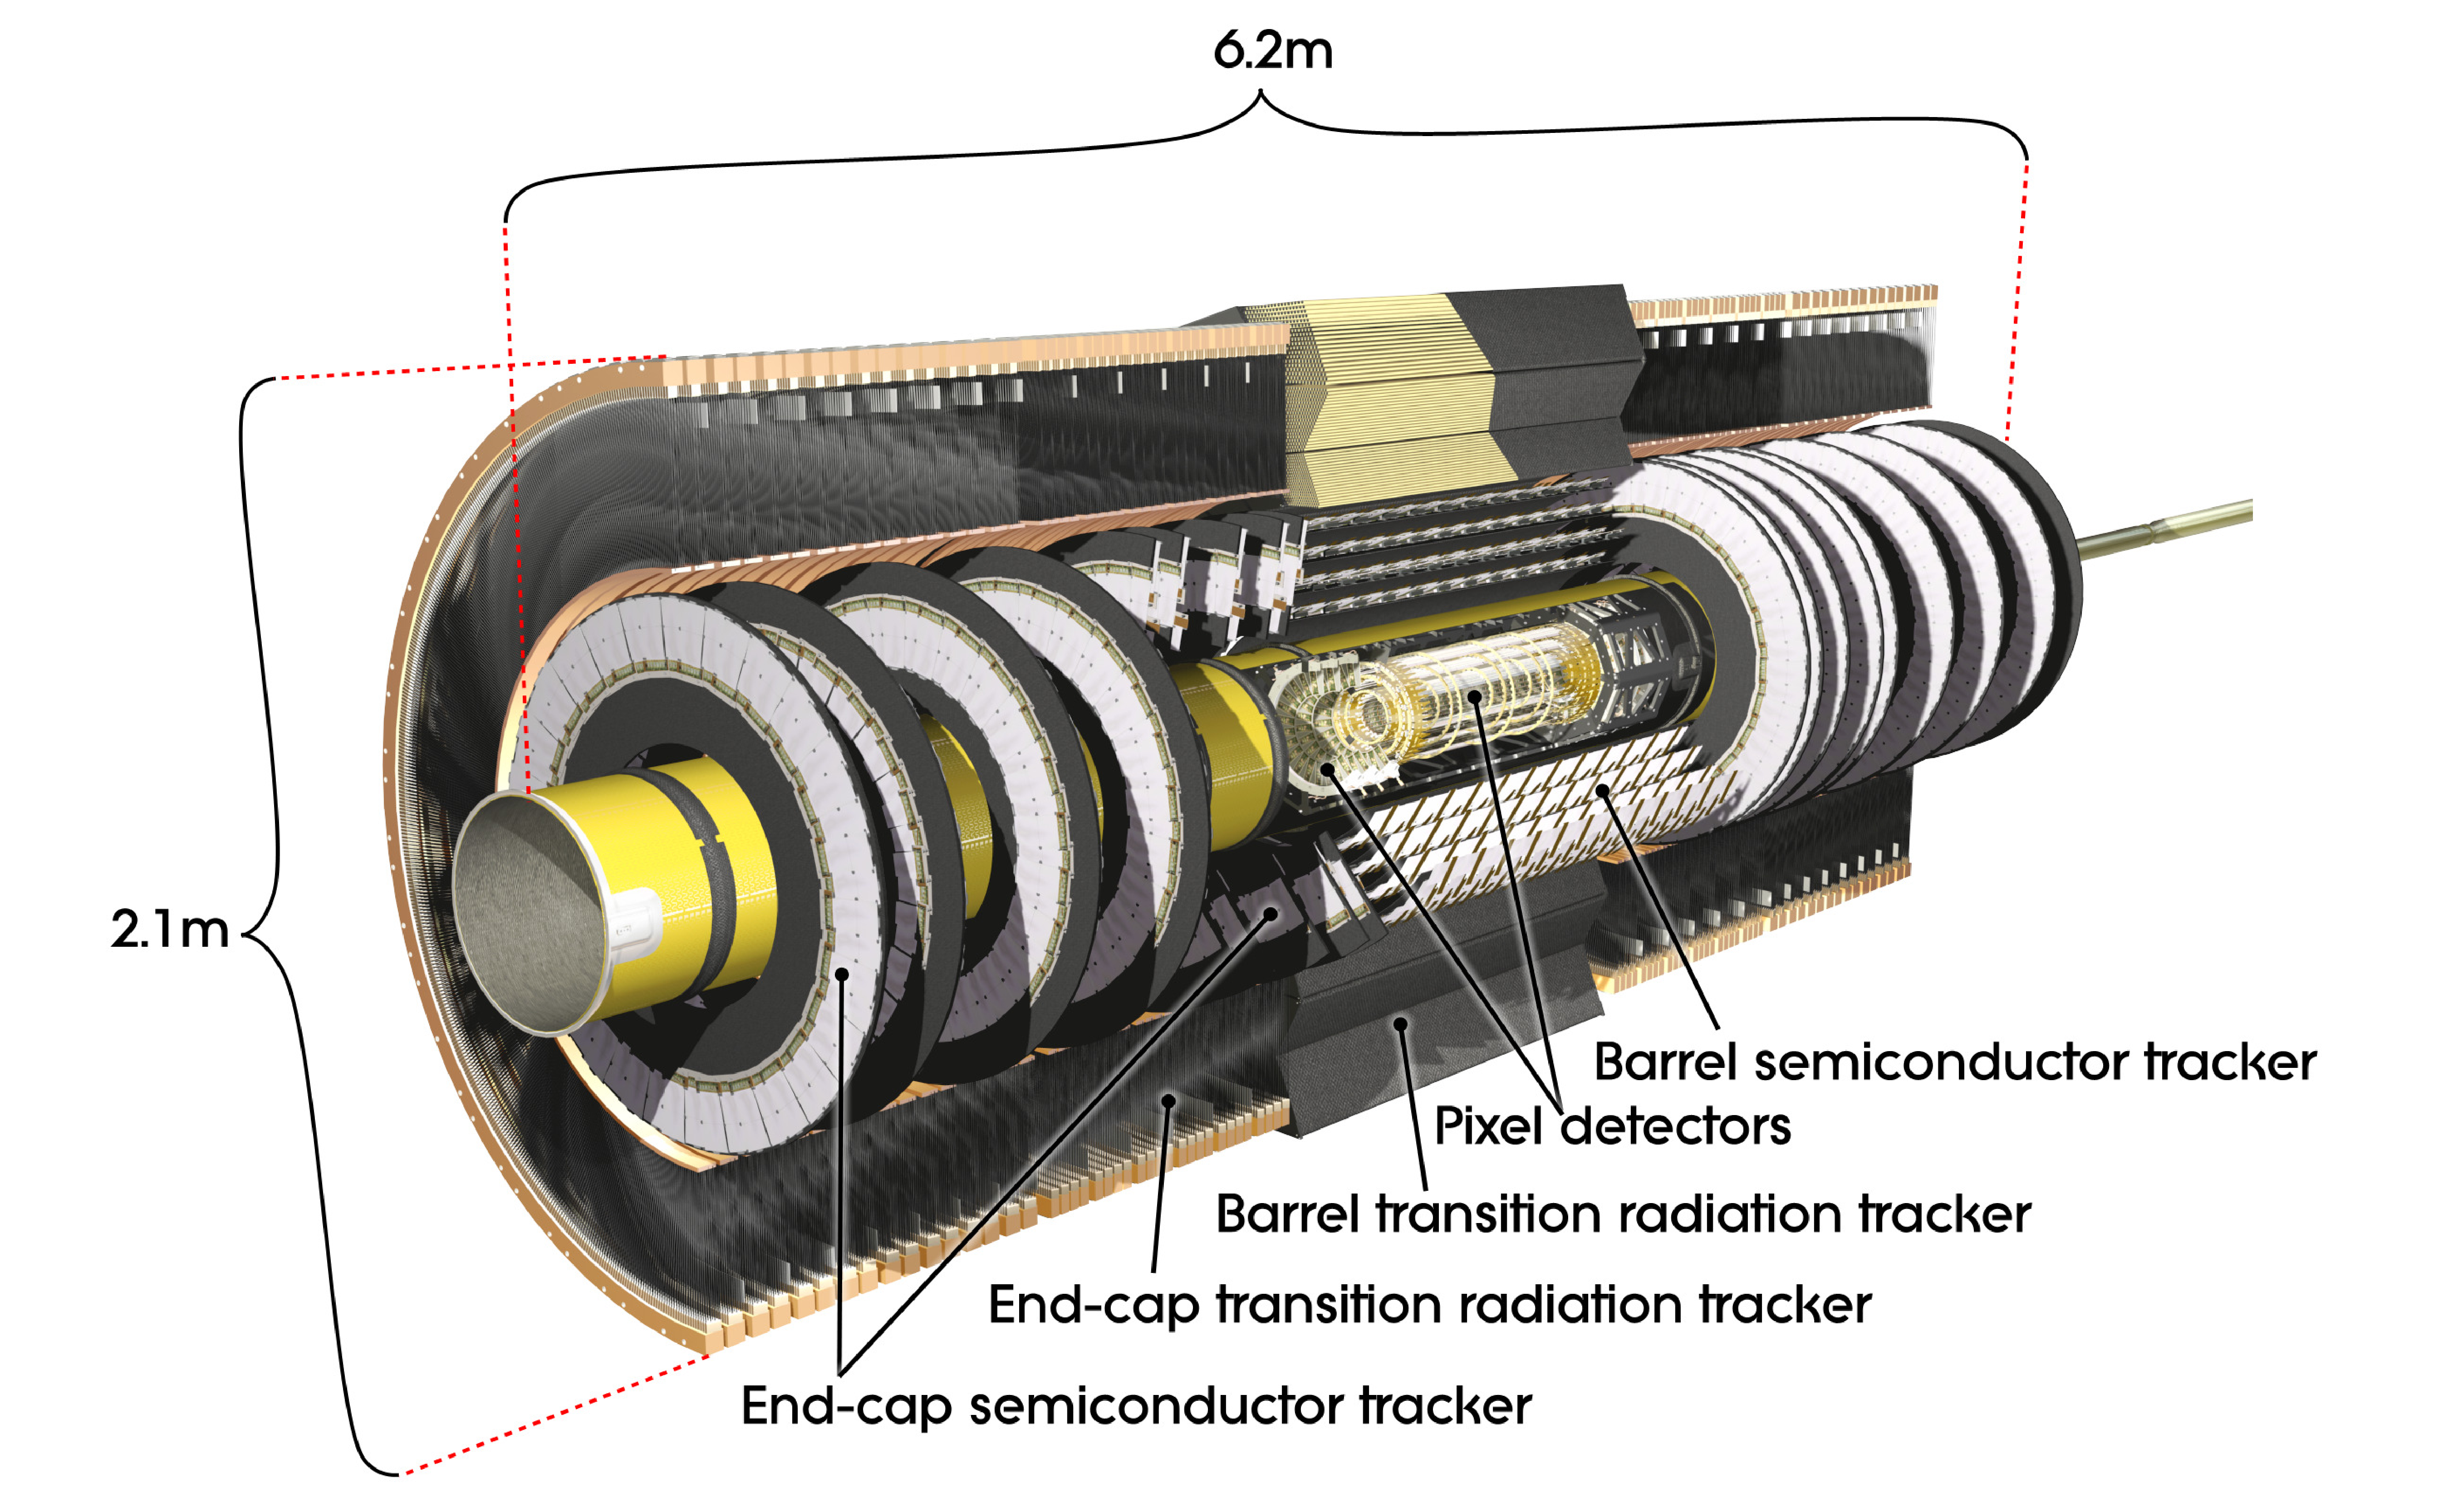
\includegraphics[width=\textwidth]{ID_newTRT_d3}
\caption{Cut-away view of the Inner Detector, taken from~\cite{Aad:1125884}.}
\label{fig:id-1}
\end{figure}

A cut-away diagram of the Inner Detector is shown in \fig{id-1}. The detector
is cylindrical in shape, extending 3512 mm either side of the interaction point
in the \z\ direction with a radius of 1150 mm. The subdetectors all consist of
concentric cylindrical layers surrounding the beam pipe, referred to as
`barrels', with disks referred to as `end caps' covering each end of the
barrels. A plan view of a quarter of the Inner Detector is shown
in~\fig{id-plan}. The Pixel and SCT detectors provide coverage up to $|\eta|<2.5$,
with the TRT enhancing pattern recognition and track momentum resoltuion up to
$|\eta|<2.0$

\begin{figure}[h]
\centering
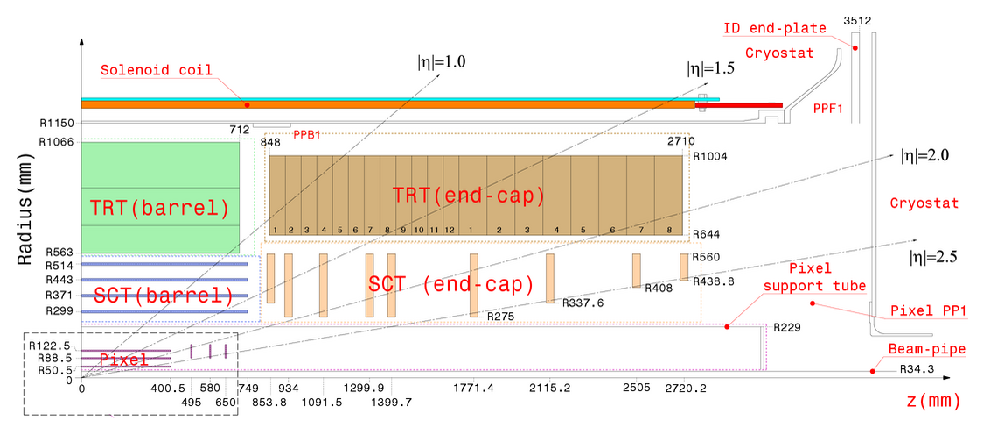
\includegraphics[width=\textwidth]{FigID26-mod-011107_crop}
\caption{Plan view of a quarter section of the Inner Dector showing the
positions and pseudo-rapidity coverage of the various subdetectors. Figure taken from~\cite{Aad:1125884}.}
\label{fig:id-plan}
\end{figure}

\subsubsection{Pixel Detector}

The pixel detector is the detector component closest to the beam. It is formed
of layers of silicon semiconducting pixels, and is designed to have a very
high granularity for resolving primary and secondary interaction vertices. There
are three barrel layers closed by an endcap consisting of three disks at each
end. The barrels are numbered from 0 to 2. The closest layer to the beam
pipe, termed the \b-layer (due to it's important role in detecting secondary
vertices for \b\ physics), is
positioned at a radius of 50.5 mm. Due to the high radiation dose that it will
recieve at this poisition, it will need to be replaced after three years
operation at design luminosity.

The detector layers are formed of sensor modules. Each module consists of a 250 \micro m thick
silicons sensor consisting of 46,080 active pixels. There are a total of 1,744
modules, all with identical dimensions of $19\times400~\mu \rm{m}^{2}$. In total
there are approximately $80.4\times 10^{6}$ readout channels.

Typically particles will traverse three layers of the detector, in most case
producing three space-points. The intrinisic accuracy of the position
measurement is 10\micro m in $(\rm{R}-\phi)$ and 155 \micro m in \z\ in the
barrel layers and 10\micro m in $(\rm{R}-\phi)$ and 155 \micro m in $\phi$ in
the endcaps.

\subsubsection{Semiconductor Tracker (SCT)}

\label{sec:Detector-SCT}

The SCT is a silicon strip detector, consisting of four barrels and two end-caps
consisting of nine disks each. The barrels consist of 2112 separate modules and
extend from a radius of 299 mm from the beam line at the innermost barrel to a
radius of 514 mm at the outermost. The barrels are numbered from 3 to 6. Each
endcap consists of 988 modules, arranged in such a way that a particle must pass
through four layers of the detector.

%SCT modules are made from two pairs of single sided p-in-n silicon chips biased
SCT modules are made from two layers of single sided p-in-n silicon chips biased
at 150V (this voltage will increase as the detector become radiation damaged). Charged particles passing through the depletion region at the centre of
the junction produce electron hole pairs, which are swept apart by the bias
voltage. The electrons are then collected on the top of the chip, producing a
signal which can be read out. A photo of an SCT barrel module is shown
in~\fig{sct-barrel-module}.

Each side of the module conists of 768 strips,
with a pitch of 80 \micro m for barrel modules, and an average picth of 80
\micro m for endcap modules. The strips are 6.4~cm long, and run parellel to the
beam axis on the barrel, and along the \R\ direction on the endcap. In total
there are approximately $6.3 \times 10^{6}$ readout channels.

% From http://atlas.web.cern.ch/Atlas/GROUPS/INNER_DETECTOR/SCT/gallery/barrel_modules/barrelmodule.jpg
% but could cite detector paper if need be
\begin{figure}[h]
\centering
\includegraphics[width=0.8\textwidth]{{SCTbarrelmodule}.jpg}
\caption{Photograph of an SCT barrel module.}
\label{fig:sct-barrel-module}
\end{figure}

%Each pair of chips is wire-bonded together and two
%pairs 
The two layers are glued together at a stereo angle of 40~mrad to form a two sided
module. The readout is of a binary form, with a charge collection threshold of 1
fC (chosen to maximise efficiency and minimise noise). To form a space-point, a
coincidence of hits on either side of the module is required. The stereo
angle gives the ability to determine where along the strip the hit occured,
giving resoltuion in \z\ (\R) in the barrels (endcaps). A small angle is used to
prevent ambiguities in the prescence of multiple nearby hits. The spatial
resolution of the detector is 17 \micro m in ($\rm{R}-\phi$) and 580 \micro m in
\z\ (in the barrel) or \R\ (in the endcaps).

\subsubsection{Transition Radition Tracker (TRT)}

The Transition Radiation Tracker is a straw drift tube tracker, with additional
particle identification capabilities from transition radiation. It consists of
modules formed from bundles of 4 mm diameter straws, filled with
$\rm{XeCO_{2}O_{2}}$ gas. A tungsten wire of 30 \micro m diameter runs down
the centre of the tube to collect charge. In the barrel the straws run parallel
with the beam axis and are 144 cm long. The wires are electrically divided into two halves at
\modetaeq{0} and read out at either end (this subdivision leads to an
inefficiency along a length of approximately 2 cm at the centre of the TRT). In
the endcaps the straws are 37 cm long and run radially. In total there are
351,000 readout channels.

% Number of hits - reolsution - advantages of continuos tracking
All charged tracks with \ptgt{0.5} and \modetalt{0.2} will travserse at least 36
straws, except in the barrel to endcap transition region (\modetabetween{0.8}{1.0})
where only 22 straws will be traversed. The ($R-\phi$) resolution is 130 \micro
m. Despite the low resolution compared to the silicon trackers, and the lack of
a measurment in the \z\ direction, the hits in the TRT contribute significantly
to the pattern recognition and momentum resolution due to the large number of
measurements and longer measured track length.

% TR
The barrel straws are embedded in a matrix of 19 \micro m diameter polypropylene
fibres, and the endcap disk layers are sandwiched between 15 \micro m
polypropylene foils. When charged particles cross these boundaries they emit
transition radition photons. These photons are then absorbed in the Xenon gas
mixture, and produce much larger signals than minimum-ionising
charged particles. The energy of the transition radiation photons depends
heavily on particle type, and is approximtaely 200 keV for a 20 GeV electron and
1 keV for a 20 GeV pion. This difference can be exploited for particle
identification, by counting the number of hits over a higher threshold.
Electrons with \ptgt{2} typically produce 7 - 10 high threshold hits, wheras
pions and other charged particles will produce far fewer.

\subsection{Calorimetery}

Sitting outside the inner detector and its magnetic field are the ATLAS
calorimeter systems. The purpose of the calorimeter is to measure the energy and
position of particles. A particle entering the calorimeter will produce a
`shower' of secondary particles. The energy of this shower is then measured.
ATLAS uses sampling calorimeter, in which differnt materials, sandwiched
together in layers, are used for the absorption and the energy measurement. This
allows for a more compact design and hence better shower containment. Position
measurement is obtained by segmenting the calorimeter in the \z\ and $\phi$
directions.

Different absorbers are required depending on whether the particle interacts
electromagnetically or strongly, and the properties of the showers that develop
are different. The ATLAS calorimeters are divided into two distinct subsystems,
the Electromagnetic calorimeter and the Hadronic calorimeter. An Electromagnetic
shower consists of electrons and photons, and is normally fully contained in the
calorimterer; thus it can be fully detected. Hadronic showers involved many more
particles types, including muons and neutrinos which escape detection, and tend
to be longer and wider, often spilling out of the calorimeter. The full energy
of the shower is thus not fully detected, and so a calibration of the energy
response is required. It is important for the calorimeter to provide good
containment for electromagnetic and hadronic showers, not only for the purposes
of energy measurement, but also to allow a goor missing transverse energy
requirement, and to prevent punch-through into the muon system.

\begin{figure}[h]
\centering
\includegraphics[width=0.9\textwidth]{{0803015_01}.jpg}
\caption{Cut-away view of the ATLAS calorimeter system. Image taken
from~\cite{1748-0221-3-08-S08003}.}
\label{fig:calo-cutaway}
\end{figure}

A cutaway view showing the location of the various calorimeter elements is shown
in~\fig{calo-cutaway}. The calorimeters cover the range \modetalt{4.9}. Over the
$\eta$ range of the inner-detector, the Electromagnetic calorimeter gives fine
granularity to allow precise measurment of electrons and photons. The Hadronic
calorimeter is more coarsely segmented, but is sufficient to meet the
requirements of jet and missing transverse energy measurement.

\subsubsection{Electromagnetic Calorimeters}

The electromagnetic calorimeter (also referred to as the {\it LAr}) uses liquid
argon as the active detector material, and lead as an absorber. Incident
particles ionise atoms in the lead absorber, creating an electromagnetic shower.
Charged particles in the shower ionise the the liquid argon, where the electrons
dirft to copper electrodes in the prescence of an electric field.

The calorimter consists of two half barrels extending to \modetalt{1.475} (with
a 4~mm gap at \z\ = 0) and two coaxial wheels on each side, the first covering
\modetabetween{1.375}{2.5} and the second covering \modetabetween{2.5}{3.2}.
Additional material needed to instrument and cool the detector creates a `crack'
region at \modetabetween{1.375}{1.52}, where the energy resolution is
significantly degraded.

The barrel calorimeter has an accordian structure in order to avoid azimuthal
cracks and to provide full $\phi$ symmetry, as shown in
figure~\fig{lar-diagram}. The accordion structure is made of
the lead absorber, with the liquid argon filling the 2.11 mm gaps between the
absorbers. The barrel of the LAr calorimeter is divided into three layers, with
different cell granularity. The first layer is divided into cells of 
\deltaetadeltaphi{0.0031}{0.098}. The fine granularity in $\eta$ of this layer
is used to determine the pseudo-rapidity of the particle, and for measurements
of the shower shape, an important input to particle identification. The
second layer has cell size \deltaetadeltaphi{0.0245}{0.025} and contains the
largest energy fraction of the shower, measuring approximately 16 radiation 
lengths. The third layer, with cell size \deltaetadeltaphi{0.0245}{0.05}, collects
the tail of the shower. The first wheel of the LAr calorimeter is also segmented into
three layers with the same granularity as the barrel. The second wheel has a
coarser granularity that varies as a function of pseudorapidity. A liquid argon
presampler exists for \modetalt{1.8} to correct for energy lost by incident
particles traversing material before the calorimeters.

%The liquid argon has to be maintained at a temperature of 88 K.

\begin{figure}[h]
\centering
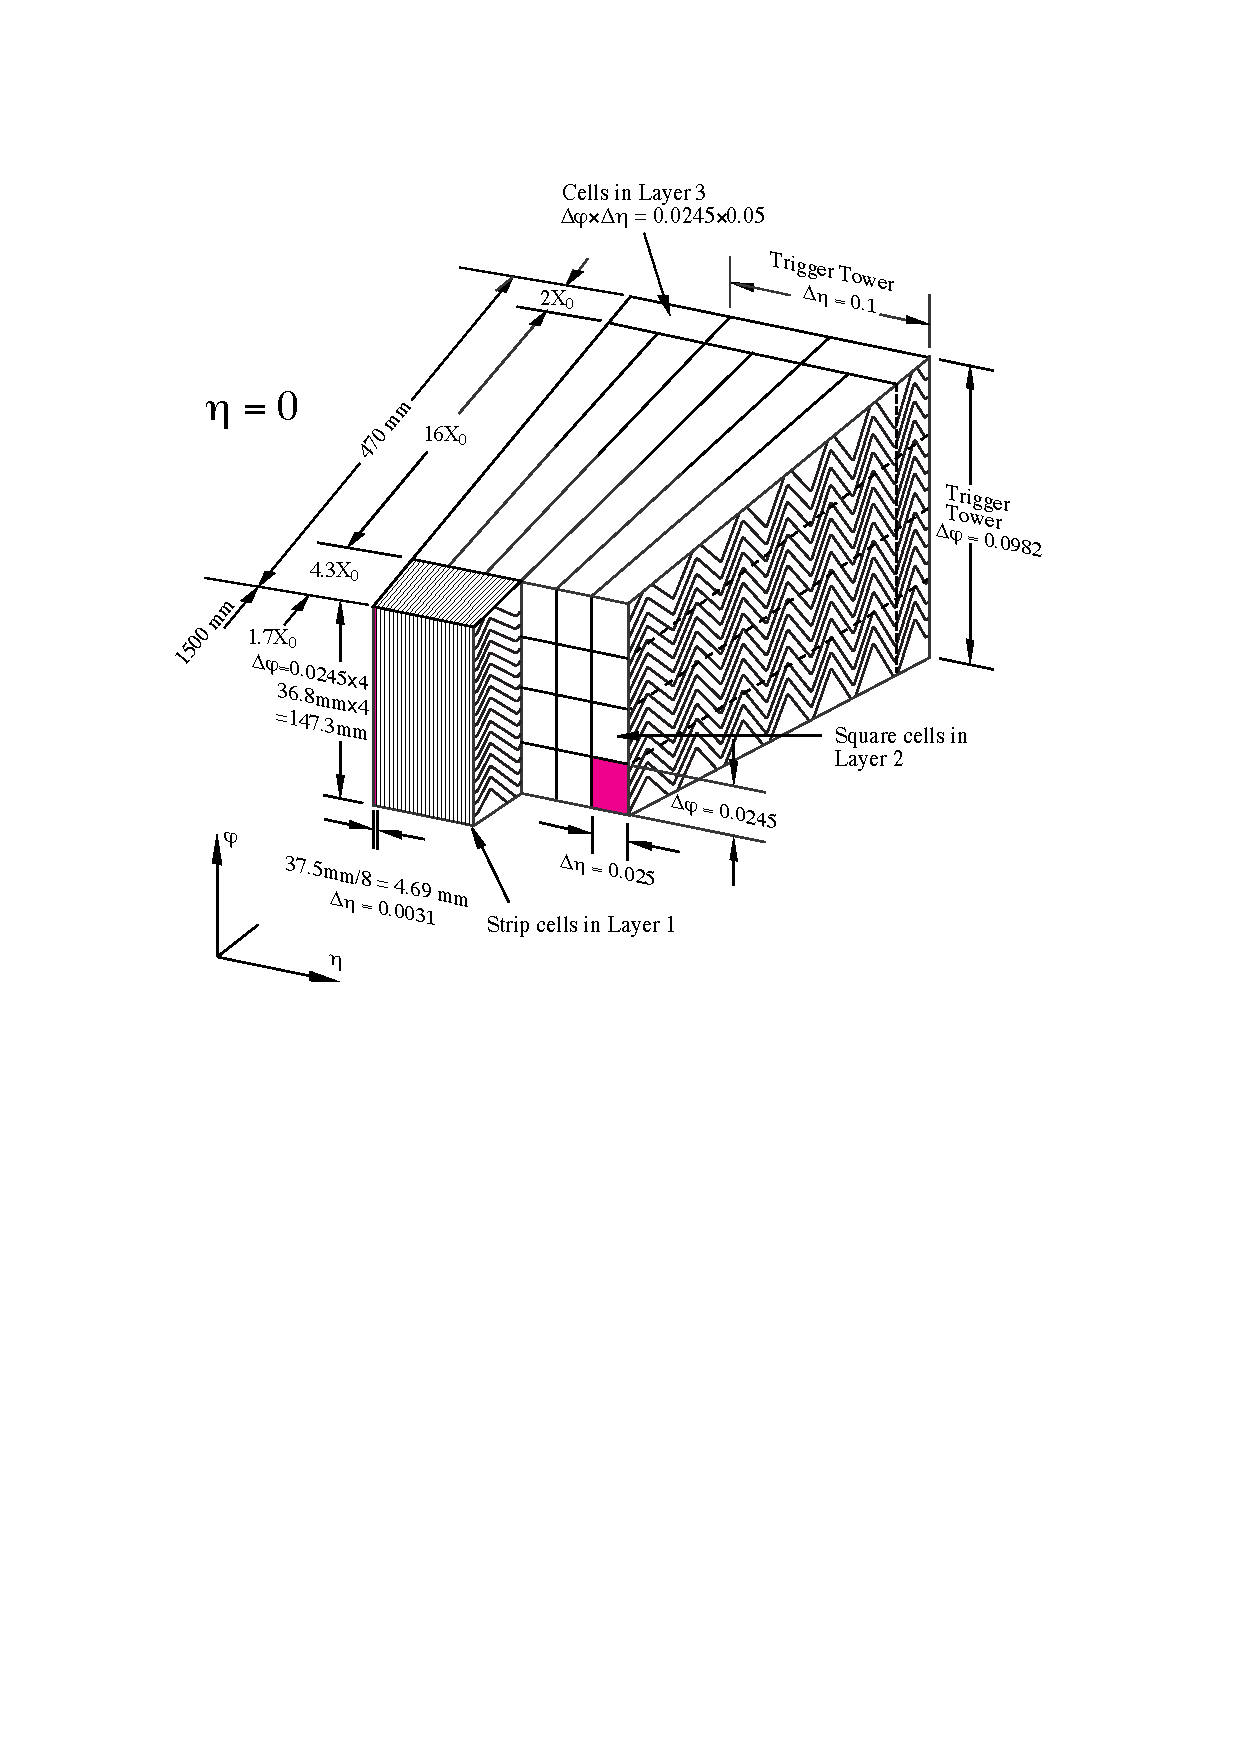
\includegraphics[width=0.8\textwidth]{lar-diagram}
\caption{Diagram of the ATLAS liquid argon calorimeter, showing the accordian
structure and the different granularity in the different layers. Diagram taken
from~\cite{1748-0221-3-08-S08003}.}
\label{fig:lar-diagram}
\end{figure}

\subsubsection{Hadronic Calorimeters}

The haronic calorimeter consists of a plastic scintillator tile calorimeter 
(referred to as the {\it Tile} calorimeter) covering \modetalt{1.7} and a liquid
argon endcap calorimeter (referred to as the {\it HEC}) coverng
\modetabetween{15}{3.2}. 

The tile calorimeter constsis of a 5.8 m long barrel covering
\modetalt{0.8} and two 2.6 m long extended barrels covering
\modetabetween{0.8}{1.7}.
It is located immediatly behind the EM calorimeter, extending from a radius of
2.28 m to a radius of 4.25 m. The active material consists of 3 mm thick layers of the plastic scintillator 
placed perpendicular to the beam direction, sandwiched between a steel absorber.
The scintillators are connected at each end to
readout photomultipliers by wavelength shifting fibres. The fibres are grouped
together to form readout cells, giving projective towers in $\eta$. There are
three layers of cells, with a granularity of \deltaetadeltaphi{0.1}{0.1} in the
first two layers, and \deltaetadeltaphi{0.1}{0.2} in the third.

The HEC consists of two wheels per endcap, HEC1 and HEC2, located directly
behind the EMEC and sharing the same cryostat. Each wheel has two layers of
cells. The HEC covers \modetabetween{1.5}{3.2} and so overlaps with the Tile
calorimeter on one side and the FCAL on the other, thus avoiding cracks in the
transition regions. HEC1 (HEC2) is built from 25 mm (50 mm) copper plate
absorbers interleaved with 8.5 mm gaps containing liquid argon. The liquid
argon gaps are split into four drift spaces of roughly 1.8 mm by three
electrodes. This is to avoid ion-build up due to the higher particles fluxes
and energies in the forward region, and also allows a lower high voltage than a single
electrode design.

\subsection{Forward Calorimeter}

The forward calorimeter ({\it FCAL}) covers \modetabetween{3.1}{4.9}. To reduce the
netron flux, the FCAL begins 1.2 m away from the Electromagnetic calorimeter
front face. Due to the high particle fluxes and energies in the forward region,
the calorimeter must contain relatively long showers in the small volume allowed
by design constraints, and thus must be very dense. The FCAL is divided into
thre compartments. The first, FCAL1, is designed for electromagnetic
measurements, and uses copper as an active material with liquid argon as a
passive material. The second two compartments, FCAL2 and FCAL3, are designed for hadronic
measurements, and use tungsten as a passive material, chosen for it's high
density to provide containment and minimise the lateral spread of hadronic
showers. An additional copper alloy shielding plate is places behind FCAL3 to
reduce background to the muon endcap system.

\subsection{Muon Spectrometer (MS)}

The muon spectrometer sits outside of the calorimeter system. It is designed to
provide precision muon momentum measurements over a momentum range of 3~GeV to
3~TeV, as well as providing triggering on interesting bunch crossings containing
muons. An overview of the MS is given in~\fig{muon-cutaway}. The system sits
inside a giant air coil toiroidal magnet system, producing a magnetic field
orthogonal to the muon momentum to provide deflection of the
muons for momentum measurement. The use of an air coil reduces multiple
scattering which degrades the momentum resolution.

\begin{figure}[h]
\centering
\includegraphics[width=0.8\textwidth]{{ms_cutaway}.jpg}
\caption{Cut away view showing the various components of the ATLAS muon
spectrometer. Figure taken
from~\cite{1748-0221-3-08-S08003}.}
\label{fig:muon-cutaway}
\end{figure}

The system consists of Monitored Drift Tubes (MDT) and Cathode Strip Chambers
(CSC) to provide precision measurements in the bending ($y-z$) plane. The MDT
covers \modetalt{2.7} and consist of three layers. The mechanical isolation of
the sensor wire in each tube from it's neighbours give a reliable system design.
In the innermost layer, for \modetabetween{2.0}{2.7} the MDT is replaced by the
CSC due to the higher rates and higher backgrounds in this region. The CSC is a
multiwire proportional chamber, and so gives a higher granularity than the MDT
and is better able to cope with high rates and fluxes.

Resistive Plate Chambers (RPC) and Thin Gap Chambers (TGC) provide triggering
for \modetalt{2.4} and a measurement in the $x-y$ plane for \modetalt{2.7}. The
RPC covers \modetalt{1.05}, with the TGC covering \modetabetween{1.05}{2.7}. The
muon trigger has a time resolution of between 1.5 ns and 4 ns.

\section{Trigger and Data Aquisition}
\section{Detector Simulation}
\section{Experiment Performance and Data Samples}

% define lb, run, period
% Luminosity graphs
% Performace of the detector over these periods
